\documentclass[12pt]{scrartcl}
\usepackage{config}
\usepackage{minted}

%\newcommand\mrh{\color{white}\bfseries}
\newcommand\mrc[1]{\begin{tabular}{@{}l@{}} #1 \end{tabular}}
\setlength\arrayrulewidth{0.8pt}

\usemintedstyle{pastie}

\begin{document}
    \hh{Arbol-stían}
    
    
    \vspace{10pt}

    
    \hh{Problem}
    
        You are given an integer $N$ and $N - 1$ bidirectional edges. These edges connect $N$ vertices in such a way that there is a path\footnote{A path is defined as a sequence of vertices, such that for any two consecutive vertices, there is an edge connecting them.} between any two vertices (i.e. they form a tree). Additionally, each vertex has a weight. For all paths, we define their weight as the product of the number of edges in it and the {\bfseries greatest common divisor} of each of the weights of the vertices in the path. Determine the simple path (a path that does not repeat edges) with the maximum weight.
    
    \hh{Implementation Details}

        You must implement the function \textit{Arbolstian()}. This function receives an integer $N$, 2 vectors $u, v$ with $N - 1$ elements, and a vector $w$, with $N$ elements. For each $0 \le i \le N - 2$, $u[i]$ and $v[i]$ are the vertices that are connected by the edge $i$. For each $0 \le i \le N - 1$, $w[i]$ is the weight of the vertex $i$. This function must return an integer, the maximum weight of a path in the tree.
        Your program should look like this:

\begin{minted}{c++}
#include <bits/stdc++.h>
using namespace std;

long long int Arbolstian(int N, vector<int> u, vector<int> v, vector<int> w) {
    // Implement this function.
}
    
\end{minted}

    The grader will call the function \textbf{multiple} times per test case.

    \hh{Examples}
    
        {\itshape Example 1:}
        \begin{itemize}
            \item The grader calls the function 
            \begin{center}
                \textit{Arbolstian(6, \{0, 0, 0, 2, 3\}, \{1, 2, 3, 4, 5\}, \{8, 2, 2, 4, 4, 8\})}
            \end{center}
            the tree in this example is illustrated in the following image:
            
            \begin{center}
                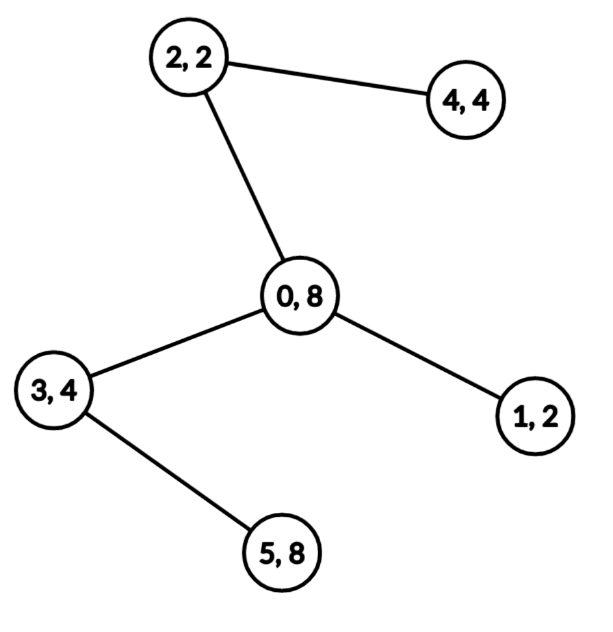
\includegraphics[scale=0.25]{ej1.png}
            \end{center}
            \item The possible paths and their weights in this tree are:
            \begin{center}
                \begin{tabular}{|c||c|c|c|c|c|c|}
                    \hline
                     $dist(a, b)$ & 0 & 1 & 2 & 3 & 4 & 5 \\
                     \hline
                     \hline
                     0 & 0 & 2 & 2 & 4 & 4 & 8 \\
                     \hline
                     1 & 2 & 0 & 4 & 4 & 6 & 6 \\
                     \hline
                     2 & 2 & 4 & 0 & 4 & 2 & 6 \\
                     \hline
                     3 & 4 & 4 & 4 & 0 & 6 & 4 \\
                     \hline
                     4 & 4 & 6 & 2 & 6 & 0 & 8 \\
                     \hline
                     5 & 8 & 6 & 6 & 4 & 8 & 0 \\ 
                     \hline
                \end{tabular}
            \end{center}
            \item The correct answer is $8$.
        \end{itemize}

        {\itshape Example 2:}
        \begin{itemize}
            \item The grader calls the function 
            \begin{center}
                \textit{Arbolstian(9, \{0, 1, 2, 3, 4, 5, 6, 7\}, \{1, 2, 3, 4, 5, 6, 7, 8\}, \{3, 3, 15, 10, 14, 7, 21, 6, 2\})}
            \end{center}
            the tree in this example is illustrated by the following image:
            \begin{center}
                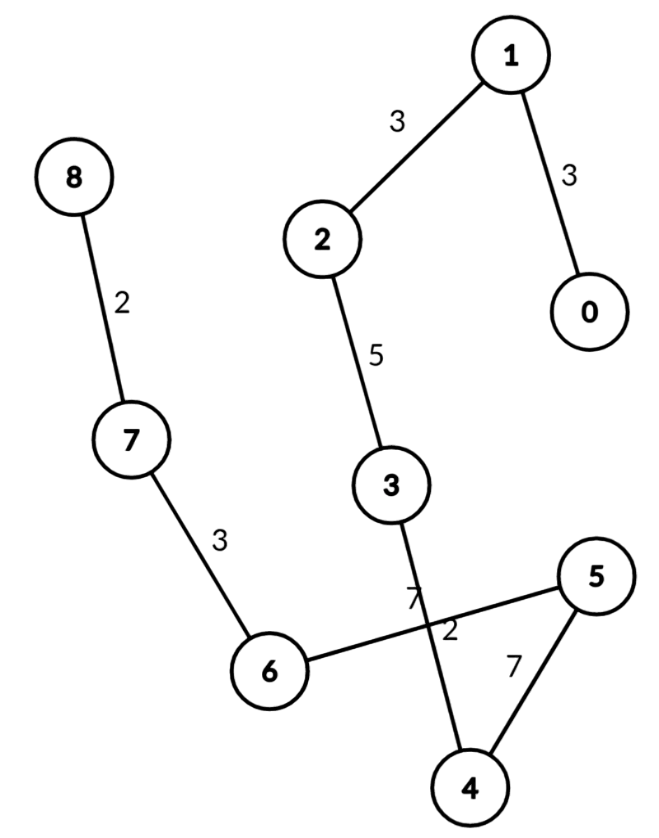
\includegraphics[scale=0.25]{ej2.png}
            \end{center}
            \item The correct answer is $14$.
        \end{itemize}
        

    \hh{Constraints}
        \begin{itemize}
            \item $1 \le N \le 2\times10^5$.
            \item The vectors $u$ and $v$ will have exactly $N - 1$ elements.
            \item The vector $w$ will have exactly $N$ elements.
            \item For each $0 \le i \le N - 2$, it holds that $0 \le u[i] \neq v[i] < N$. 
            \item For each $0 \le i \le N - 1$, it holds that $1 \le w[i] \le 10^6$.
            \item It is guaranteed that the graph formed by the edges is a tree.
            \item Let $S_N$ be the sum of all values of $N$ across all function calls. It is guaranteed that $S_N \le 2\times 10^5$.
        \end{itemize}
    
    \hh{Subtasks}


    \begin{itemize}
        \item (3 points) $N, S_N \le 2000$.
        \item (9 points) For all $0 \le i \le N - 1$, it holds that $w[i] = 1$.
        \item (11 points) For all $0 \le i \le N - 2$, it holds that $\gcd(w[u[i]], w[v[i]])$ is a prime number.
        \item (22 points) For all $0 \le i \le N - 1$, it holds that $w[i]$ is a power of 2.
        \item (22 points) For all $0 \le i \le N - 2$, it holds that $u[i] = i, v[i] = i + 1$.
        \item (33 points) No additional restrictions.
    \end{itemize}
\end{document}
